\documentclass[12pt]{article}
\usepackage[utf8]{inputenc}
\usepackage{longtable}
\usepackage{color}
\usepackage{multirow}
\usepackage{hyperref}
\usepackage{amssymb}
\usepackage{setspace}
%\doublespacing

\renewcommand*{\sectionautorefname}{Section} 

\title{Predation model \\ Hybridisation} 
\author{Raphael Klein, EPFL}

\usepackage{natbib}
\usepackage{graphicx}
\usepackage[labelfont=bf]{caption} 	% Make captions bold (Figure & Table)
\usepackage{subfig}	
\usepackage{amsmath}
\usepackage{hyperref}
%\usepackage[section]{placeins}

\providecommand{\keywords}[1]{\textbf{Keywords:} #1}

\begin{document}

\maketitle

%\textcolor{red.green.blue.cyan.yellow.magenta.}{}

%%%%%%%%%%%%%%%%%%%%%%%%%%%%%%%%%%%%%%%%%%%%%%%%%%%%%%%%%%%%%%%%%%
\section{The problem tree}
\label{sec:interfaceProblemTree}
%%%%%%%%% %%%%%%%%%%%%%%%%%%%%%%%%%%

Overall, the problem tree is given as follows:

\begin{itemize}
\item Policy core problems:
	\begin{enumerate}
	
	\item Sheep - 
	The amount of sheep on the grid.
	
	\item Wolf - 
	The amount of wolves on the grid.
	
	\item Fully grown grass - 
	The amount of fully grown grass on the grid.
	
	\end{enumerate}
	
\item Secondary problems:
	\begin{enumerate}

	\item Net sheep population change - 
	This is the difference between initial and final amount of sheep.
	
	\item Net wolf population change - 
	This is the difference between initial and final amount of wolves.
	
	\item Net grown grass patch change - 
	This is the difference between initial and final amount of grown grass patches.
	
	\end{enumerate}
	
\end{itemize}

Note that the secondary issues and the policy core issues are the same. The main reason behind this choice is the simplicity of the model. The model is so simple that the it is difficult to find any different policy core issues.

%%%%%%%%%%%%%%%%%%%%%%%%%%%%%%%%%%%%%%%%%%%%%%%%%%%%%%%%%%%%%%%%%%
\section{The policy instruments}
\label{sec:interfaceInstruments}
%%%%%%%%% %%%%%%%%%%%%%%%%%%%%%%%%%%

The policy instruments within the policy tree are implemented using incremental increases and decreases in the following exogenous parameters.

\begin{enumerate}
\item Change sheep reproduction [CR-0.01/+0.01]
\item Change wolf reproduction [WR -0.01/+0.01]
\item Change grass regrowth [GR-2/+2]
\end{enumerate}



%%%%%%%%%%%%%%%%%%%%%%%%%%%%%%%%%%%%%%%%%%%%%%%%%%%%%%%%%%%%%%%%%%
\section{The steps for model integration}
\label{sec:steps}
%%%%%%%%% %%%%%%%%%%%%%%%%%%%%%%%%%%

This section presents the steps that are needed to connect a policy context model, in this case the predation model, to the policy process model.

\begin{enumerate}
\item Before any coding, define what the belief tree and the policy instruments will be for the predation model.
\item Copy the policy emergence model files into the same folder.
\item In \texttt{runbatch.py}, replace the policy context items by the predation model.
\item In \texttt{runbatch.py}, make sure to initialise the predation model appropriately.
\item Change the \texttt{input goalProfiles} files to have the appropriate belief tree structure of the predation model.
\item In \texttt{model module interface.py}, construct the belief tree and the policy instrument array.
\item Make sure that the step function in the \texttt{model predation.py} returns the KPIs that will fit in the belief system in the order DC, PC and S. If no DC is considered, then include one value of 0 at least. All KPIs need to be normalised.
\item Modify the step function of the \texttt{model predation.py} to include a policy implemented.
\item Introduce the changes that a policy implemented would have on the model in \texttt{model predation.py}.
\end{enumerate}


%%%%%%%%%%%%%%%%%%%%%%%%%%%%%%%%%%%%%%%%%%%%%%%%%%%%%%%%%%%%%%%%%%
\section{The steps for model simulation}
\label{sec:steps}
%%%%%%%%% %%%%%%%%%%%%%%%%%%%%%%%%%%

This section presents the steps that are needed to connect a policy context model, in this case the predation model, to the policy process model.

\begin{enumerate}
\item For the policy process:
	\begin{enumerate}
	\item Define a set of hypotheses to be tested
	\item Define scenarios that will be needed to assess the hypotheses
	\item Choose the agent distribution based on the scenarios constructed
	\item Set the preferred states for the active agents and the electorate along with the causal beliefs to be used. This should all be based on the scenarios that have been constructed.
	\end{enumerate}

\item For the predation model:
	\begin{enumerate}
	\item Define the initial values for the main parameters
	\item Define the parameters that will be recorded
	\end{enumerate}
\item Save the right data from the model.
\end{enumerate}

%%%%%%%%%%%%%%%%%%%%%%%%%%%%%%%%%%%%%%%%%%%%%%%%%%%%%%%%%%%%%%%%%%
\section{Model hypotheses}
\label{sec:steps}
%%%%%%%%% %%%%%%%%%%%%%%%%%%%%%%%%%%

Several hypotheses are made for testing the policy process model. They are given as follows:

\begin{itemize}
\item H1: The introduction of the policy emergence model will affect the Schelling model outcomes.
\item H2: The change of decision making power balance will lead to policy change.
\item H3: A sudden change in the preferred states of the policy agents will lead to policy change.
\item H4: The electorate has a long term impact on policy change.
\item H5: A change in the system's understanding impacts policy selection.
\end{itemize}

%%%%%%%%%%%%%%%%%%%%%%%%%%%%%%%%%%%%%%%%%%%%%%%%%%%%%%%%%%%%%%%%%%
\section{Model scenarios}
\label{sec:steps}
%%%%%%%%% %%%%%%%%%%%%%%%%%%%%%%%%%%

Six scenario are considered. All but one focus on a change in the preferred states of the agents or their causal beliefs. For each of the scenario, the preferred states of the agents are shown in \autoref{tab:preferredStates} and their causal relations are provided in \autoref{tab:causalBeliefs}.

% max sheep: [0, 500]
% max wolves: [0, 500]
% mass grass patches: [2500]
% Net sheep population change: [-100; 100]
% Net wolf population change: [-100; 100]
% Net grown grass patch change: [-500; 500]

\begin{table}[h!]
\begin{center}
\begin{tabular}{ |c|c|c|c|c|c|c| } 
\hline

			& PC1	& PC2	& PC3	& S1		& S2		& S3  	\\ 
			& Sheep	& Wolves	& Grass	& Sheep	& Wolves	& Grass 	\\
			&		&		&		& growth	& growth	& growth	\\ \hline
			
\multicolumn{7}{|c|}{Scenario 0}										\\ \hline
Policy makers	& 300	& 300	& 2000	& 100	& 50		& 200	\\ \hline
			& 0.60	& 0.60	& 0.80	& 1.00	& 0.75	& 0.70	\\ \hline
			
\multicolumn{7}{|c|}{Scenario 1}										\\ \hline
Policy makers	& 150	& 0		& 2000	& 100	& 50		& 200	\\ \hline
			& 0.30	& 0.00	& 0.80	& 1.00	& 0.75	& 0.70	\\ \hline
			
\multicolumn{7}{|c|}{Scenario 2}										\\ \hline
Policy makers	& 300	& 300	& 2000	& 50		& -25	& 100	\\ \hline
			& 0.60	& 0.60	& 0.80	& 0.75	& 0.38	& 0.60	\\ \hline

\multicolumn{7}{|c|}{Scenario 3}										\\ \hline
Policy makers	& 300	& 300	& 2000	& 100	& 50		& 200	\\ \hline
			& 0.60	& 0.60	& 0.80	& 1.00	& 0.75	& 0.70	\\ \hline
			
\multicolumn{7}{|c|}{Scenario 4}										\\ \hline
Policy makers	& 300	& 300	& 2000	& 100	& 50		& 200	\\ \hline
			& 0.60	& 0.60	& 0.80	& 1.00	& 0.75	& 0.70	\\ \hline
Electorate		& 150	& 0		& 2000	& 100	& 50		& 200	\\ \hline
			& 0.30	& 0.00	& 0.80	& 1.00	& 0.75	& 0.70	\\ \hline


\multicolumn{7}{|c|}{Scenario 5}										\\ \hline
Policy makers	& 300	& 300	& 2000	& 100	& 50		& 200	\\ \hline
			& 0.60	& 0.60	& 0.80	& 1.00	& 0.75	& 0.70	\\ \hline
Electorate		& 300	& 300	& 2000	& 50		& -25	& 100	\\ \hline
			& 0.60	& 0.60	& 0.80	& 0.75	& 0.38	& 0.60	\\ \hline

\end{tabular}
\end{center}
\caption{Preferred states for the policy makers on a the interval [0,1].}
\label{tab:preferredStates}
\end{table}

\begin{table}[h!]
\begin{center}
\begin{tabular}{ |c|c|c|c| |c|c|c|c|}
 \hline
\multicolumn{4}{|c||}{Scenario 0/1/2/4/5}	& \multicolumn{4}{|c|}{Scenario 3}		\\ \hline
	& PC1	& PC2	& PC3		& 		& PC1	& PC2	& PC3	\\ \hline
-S1 	& 1.00	& 0.75	&-0.75		& -S1 	&-0.50	&-0.10	& 0.25	\\ \hline
-S2 	&-0.75	& 1.00	& 0.25 		& -S2 	& 0.05	&-0.50	&-0.25 	\\ \hline
-S3 	& 0.50	& 0.75	& 1.00		& -S3 	&-0.25	& 0.00	&-0.50	\\ 
 \hline
\end{tabular}
\end{center}
\caption{Causal beliefs for the policy makers. These causal relations can be read as: an increase of 1 in S2 will lead to a decrease of 0.75 in PC1. They are all given on the interval [-1,1].}
\label{tab:causalBeliefs}
\end{table}

\begin{itemize}
\item Scenario 0 - Benchmark

The benchmark scenario is to be used as a benchmark. It is a simulation of the predation model with the policy emergence model. The preferred states for the agents is provided in \autoref{tab:preferredStates}. The causal beliefs used as given in \autoref{tab:causalBeliefs}.

\item Scenario 1 - Change in the policy core issue preferred states

Scenario 1 looks at what would change if the policy core issue preferred states of the policy makers were different. The new selection of preferred states is given in \autoref{tab:preferredStates}.

\item Scenario 2 - Change in the secondary issue preferred states

Scenario 2 looks at what would change if the secondary issue preferred states of the policy makers were different. The new selection of preferred states is given in \autoref{tab:preferredStates}.

\item Scenario 3 - Change in the causal beliefs

For Scenario 3, we compare a difference in the understanding of how the system works and its impact on policy change. For this we create a different causal beliefs structure that is presented in \autoref{tab:causalBeliefs}. This is to be compared with results from the benchmark in scenario 0.

\item Scenario 4 \& 5 - Electorate influence on the policy core and secondary issue preferred states

For scenario 3, we also check what is the impact of different electorate influence weight values. The aim is to visualise the impact of the influence electorate on the overall system for this. We have the same scenario as for scenario 2 but this time the electorate is much more driven and has a quick impact on the policy makers (quadrupling to 0.20 their influence on policy makers). The weights considered are 0.20, 0.02 and 0.50.

\end{itemize}


%%%%%%%%%%%%%%%%%%%%%%%%%%%%%%%%%%%%%%%%%%%%%%%%%%%%%%%%%%%%%%%%%%
\section{Initialisation of the predation model}
\label{sec:predation_initialisation}
%%%%%%%%%%%%%%%%%%%%%%%%%%%%%%%%%%%

The parameters that need to be initialised for the predation model are given by:

\begin{itemize}
\item Grid height: 50
\item Grid width: 50
\item Initial amount of grass: about 50\% of the grid
\item Initial number of sheep: 250
\item Sheep reproduce rate: 4\%
\item Sheep gain from food: 6
\item Initial number of wolves: 25
\item Wolf reproduce rate: 5\%
\item Wolf gain from food: 35
\item Grass regrowth time: 30
\end{itemize}

Note that the initial parameter as chosen such that if only the predation model is run, it has a stable configuration. Furthermore the onus is placed on the simulation of the policy process, therefore no scenarios are placed on the predation model side of the simulation.


%%%%%%%%%%%%%%%%%%%%%%%%%%%%%%%%%%%%%%%%%%%%%%%%%%%%%%%%%%%%%%%%%%
\section{Results}
\label{sec:results}
%%%%%%%%%%%%%%%%%%%%%%%%%%%%%%%%%%%

The results section is divided up into the different hypotheses that were brought up previously.

\subsection{On hypothesis 1}
\label{ssec:H1}
%%%%%%%%%%%%%%%%%%%%%%%%%%%%%%%%%%%

\emph{The introduction of the policy emergence model will affect the Schelling model outcomes.}

\begin{figure}[ht]
\centering
\includegraphics[width=\linewidth]{figures/Predation_SM_Comparisons_Scenarios.eps}
\caption{Comparison of the results from the predation model for all scenarios plus the predation model without policy emergence model.}
\label{fig:Predation_SM_Comparisons_Scenarios}
\end{figure}

Clearly they have an effect. They have a destabilising effect on the model. As the distributions show, the wolf and sheep concentration are closer together when the policy actors intervene based on their goals and beliefs.

\subsection{On hypothesis 2}
\label{ssec:H2}
%%%%%%%%%%%%%%%%%%%%%%%%%%%%%%%%%%%

\emph{The change of decision making power balance will lead to policy change.}

%\begin{figure}[ht]
%\centering
%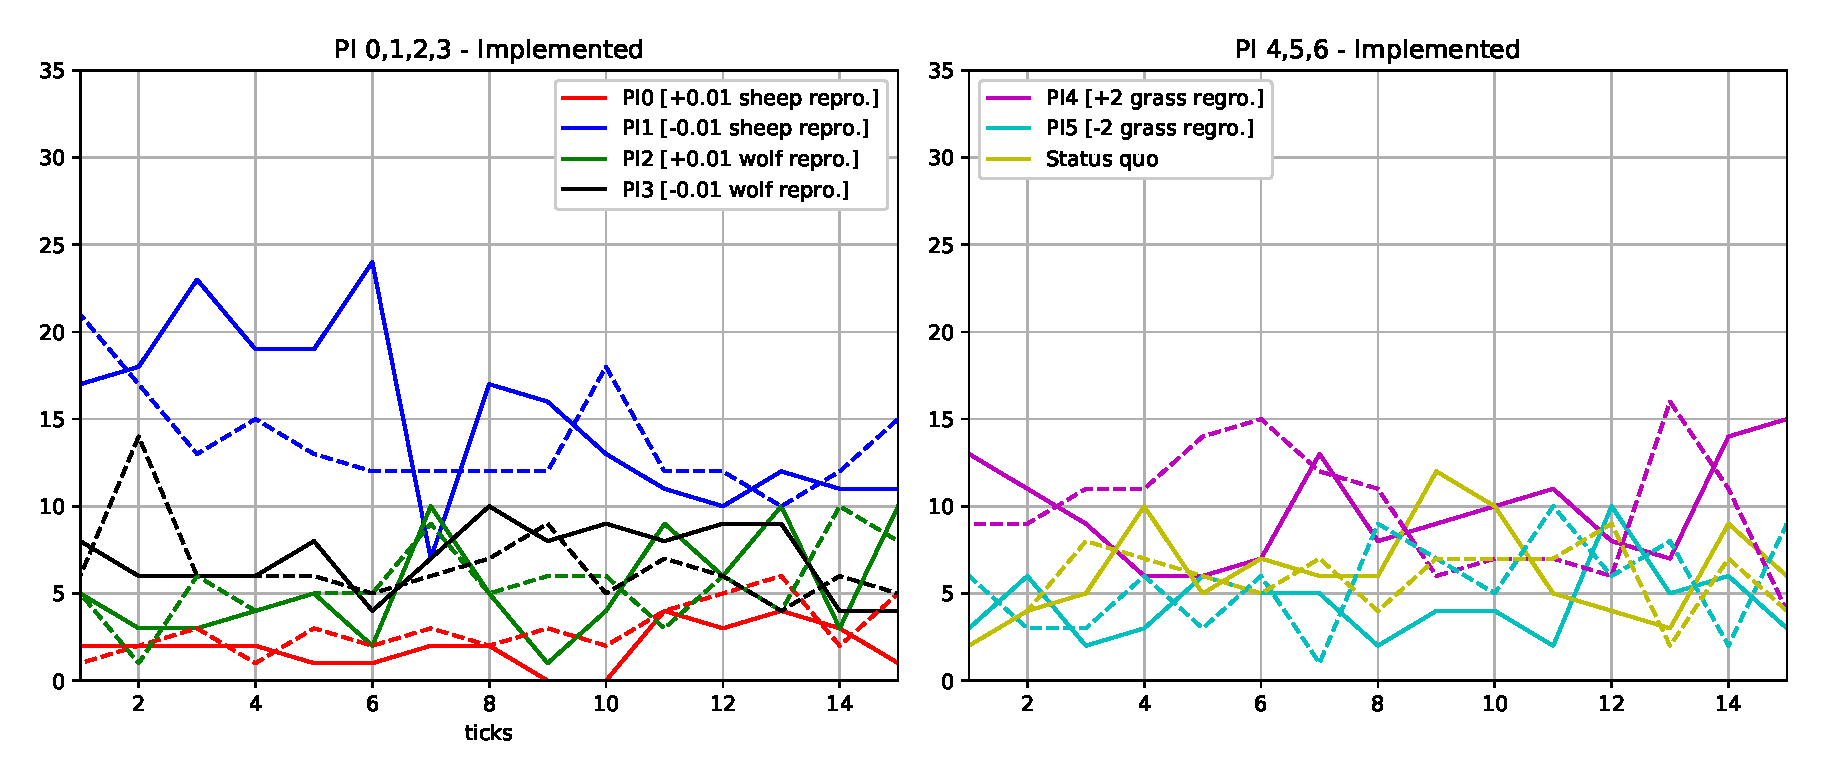
\includegraphics[width=\linewidth]{figures/PE_PI_Comparison_Implemented_Sce0-1}
%\caption{Policy instruments implemented over time. Scenario 1 is the full line and scenario 2 is the dashed line.}
%\label{fig:PE_PI_Comparison_Implemented_Sce0-1}
%\end{figure}

\subsection{On hypothesis 3}
\label{ssec:H3}
%%%%%%%%%%%%%%%%%%%%%%%%%%%%%%%%%%%

\emph{A sudden change in the preferred states of the policy agents will lead to policy change.}

Plot the right scenario for this - Scenario 4

%\begin{figure}[ht]
%\centering
%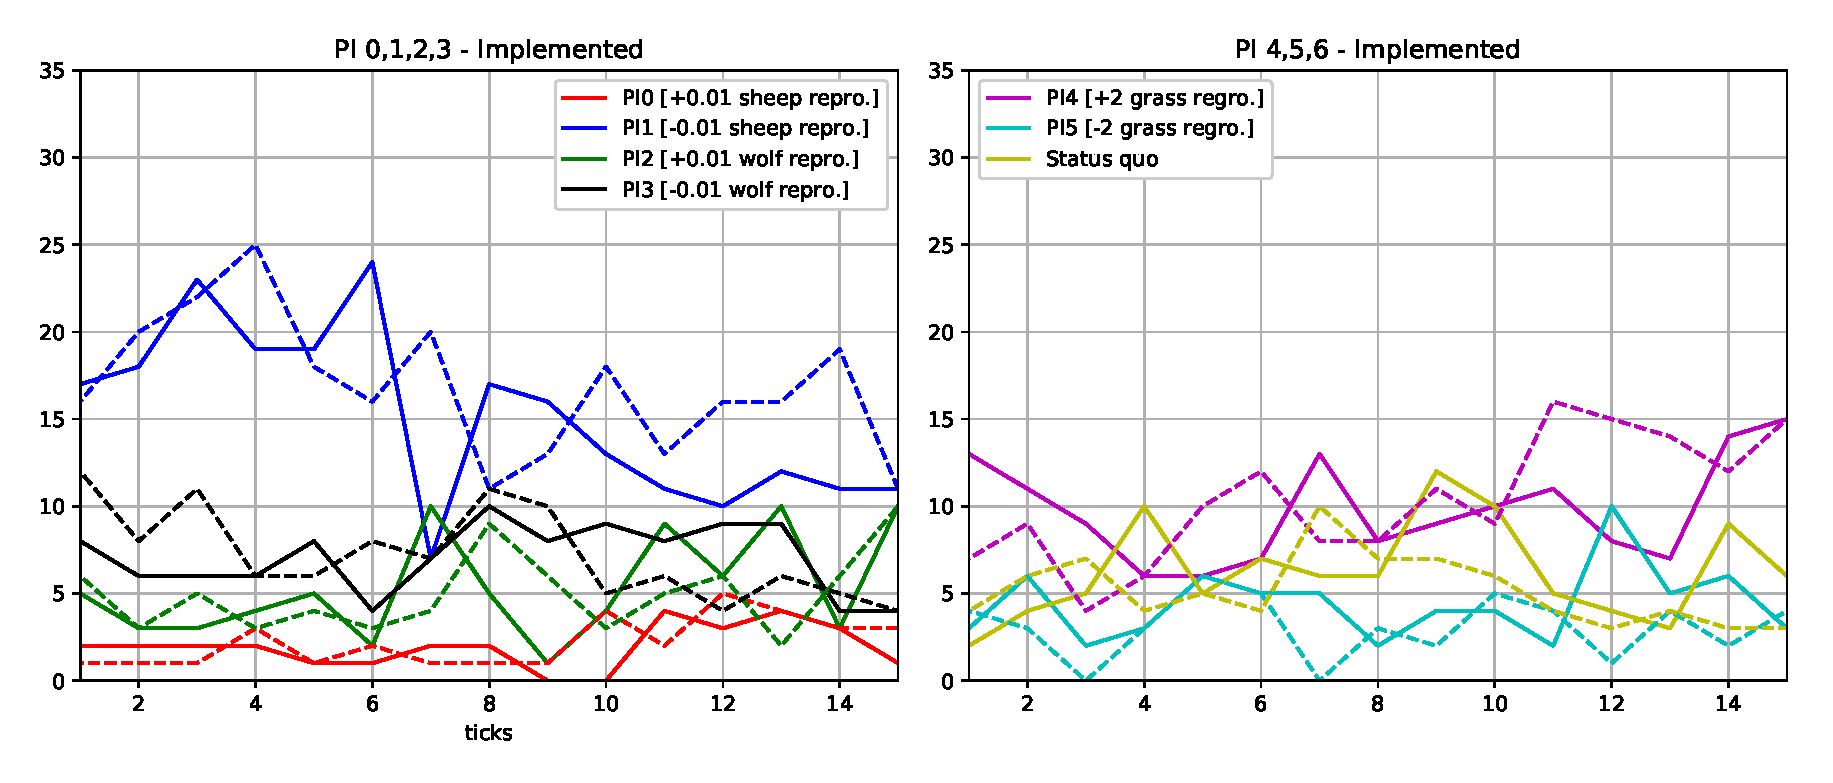
\includegraphics[width=\linewidth]{figures/PE_PI_Comparison_Implemented_Sce0-2}
%\caption{Policy instruments implemented over time. Scenario 1 is the full line and scenario 3 is the dashed line.}
%\label{fig:PE_PI_Comparison_Implemented_Sce0-2}
%\end{figure}

\subsection{On hypothesis 4}
\label{ssec:H4}
%%%%%%%%%%%%%%%%%%%%%%%%%%%%%%%%%%%

\emph{The electorate has a long term impact on policy change.}

%\begin{figure}[ht]
%\centering
%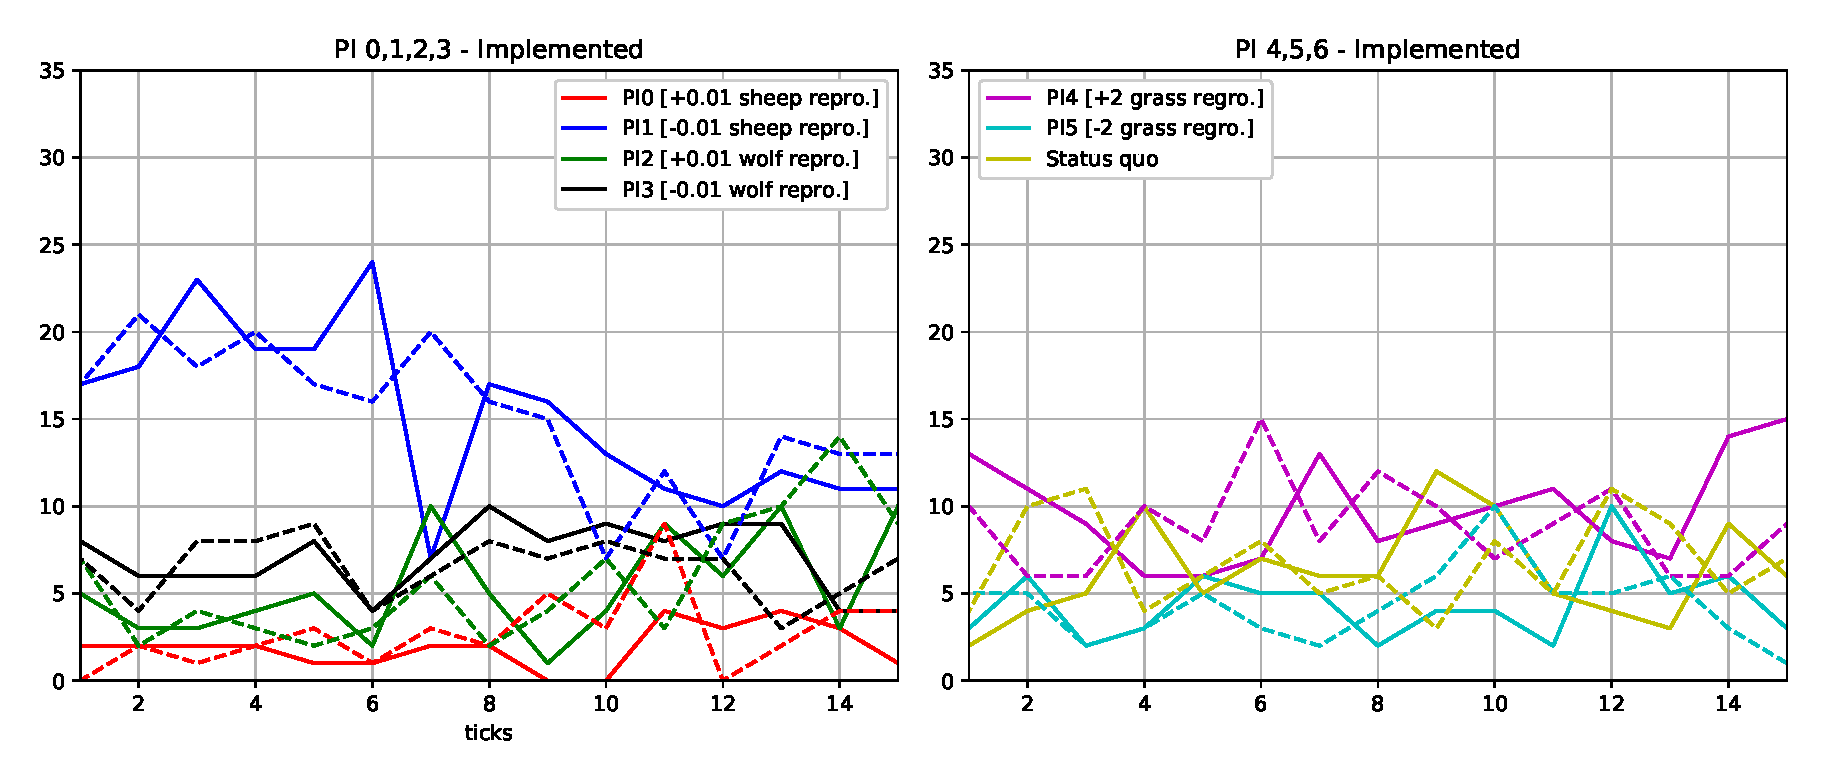
\includegraphics[width=\linewidth]{figures/PE_PI_Comparison_Implemented_Sce0-3}
%\caption{Policy instruments implemented over time. Scenario 1 is the full line and scenario 4 is the dashed line.}
%\label{fig:PE_PI_Comparison_Implemented_Sce0-3}
%\end{figure}

%%%%%%%%%%%%%%%%%%%%%%%%%%%%%%%%%%%%%%%%%%%%%%%%%%%%%%%%%%%%%%%%%%
\bibliographystyle{apalike} 
\bibliography{references}
%%%%%%%%%%%%%%%%%%%%%%%%%%%%%%%%%%%%%%%%%%%%%


\end{document}
